% fig0_overview.tex -- symbolic TikZ schematic of the reliability-collapse audit design.
% Standalone build (own Makefile target `fig0`); NOT part of the R figure
% pipeline (which regenerates F1--F6 from on-disk result JSONs). Compile with:
%   pdflatex -interaction=nonstopmode -halt-on-error fig0_overview.tex
% Native width is held under the narrower of the two venue textwidths
% (sn-jnl/DMKD: 372pt = 13.07cm) so \includegraphics never has to shrink the
% embedded 8pt node text below the print floor in either paper.tex or
% paper_svjour.tex.
\documentclass[tikz,border=1pt]{standalone}
\usetikzlibrary{arrows.meta,positioning,fit,backgrounds}

% Okabe-Ito colorblind-safe palette (matches figures/ggtheme.R).
\definecolor{oiBlue}{HTML}{0072B2}
\definecolor{oiOrange}{HTML}{E69F00}
\definecolor{oiGreen}{HTML}{009E73}
\definecolor{oiVermillion}{HTML}{D55E00}
\definecolor{oiGrey}{HTML}{595959}

% -- Small TikZ pictograms (shapes only, no photographic assets) used in place
% of text-heavy box content; each is a self-contained mini tikzpicture sized
% to sit on its own line above a short label inside a node.
\newcommand{\iconDB}{\tikz[baseline=-0.5ex]{
  \draw[oiGrey,thick] (0,0.9mm) ellipse (2.3mm and 0.8mm);
  \draw[oiGrey,thick] (-2.3mm,0.9mm) -- (-2.3mm,-2mm);
  \draw[oiGrey,thick] (2.3mm,0.9mm) -- (2.3mm,-2mm);
  \draw[oiGrey,thick] (-2.3mm,-2mm) arc (180:360:2.3mm and 0.8mm);}}
\newcommand{\iconSplit}[1]{\tikz[baseline=-0.5ex]{
  \draw[#1,thick] (0,-1.6mm) -- (0,0);
  \draw[#1,-{Latex[length=1.2mm,width=1mm]},thick] (0,0) -- (-1.9mm,1.7mm);
  \draw[#1,-{Latex[length=1.2mm,width=1mm]},thick] (0,0) -- (1.9mm,1.7mm);}}
\newcommand{\iconLock}{\tikz[baseline=-0.5ex]{
  \draw[oiGrey,thick] (-1.6mm,-1.7mm) rectangle (1.6mm,0.5mm);
  \draw[oiGrey,thick] (-1mm,0.5mm) arc (180:0:1mm and 1.5mm);}}
\newcommand{\iconLadder}{\tikz[baseline=-0.5ex]{
  \draw[oiGrey,thick] (-1.8mm,-2mm) -- (-1.8mm,2mm);
  \draw[oiGrey,thick] (1.8mm,-2mm) -- (1.8mm,2mm);
  \draw[oiGrey,thick] (-1.8mm,-1.1mm) -- (1.8mm,-1.1mm);
  \draw[oiGrey,thick] (-1.8mm,0mm) -- (1.8mm,0mm);
  \draw[oiGrey,thick] (-1.8mm,1.1mm) -- (1.8mm,1.1mm);}}
\newcommand{\iconGauge}{\tikz[baseline=-0.5ex]{
  \draw[oiGrey,thick] (-2.2mm,0) arc (180:0:2.2mm);
  \draw[oiGrey,thick] (0,0) -- (-1.3mm,1.6mm);
  \draw[oiGrey,thick] (-2.2mm,0) -- (2.2mm,0);}}
\newcommand{\iconCheck}{\tikz[baseline=-0.5ex]{
  \draw[oiGreen,line width=1pt] (-1.7mm,0) -- (-0.3mm,-1.5mm) -- (1.9mm,1.7mm);}}
\newcommand{\iconCross}{\tikz[baseline=-0.5ex]{
  \draw[oiVermillion,line width=1pt] (-1.5mm,-1.5mm) -- (1.5mm,1.5mm);
  \draw[oiVermillion,line width=1pt] (-1.5mm,1.5mm) -- (1.5mm,-1.5mm);}}

\begin{document}
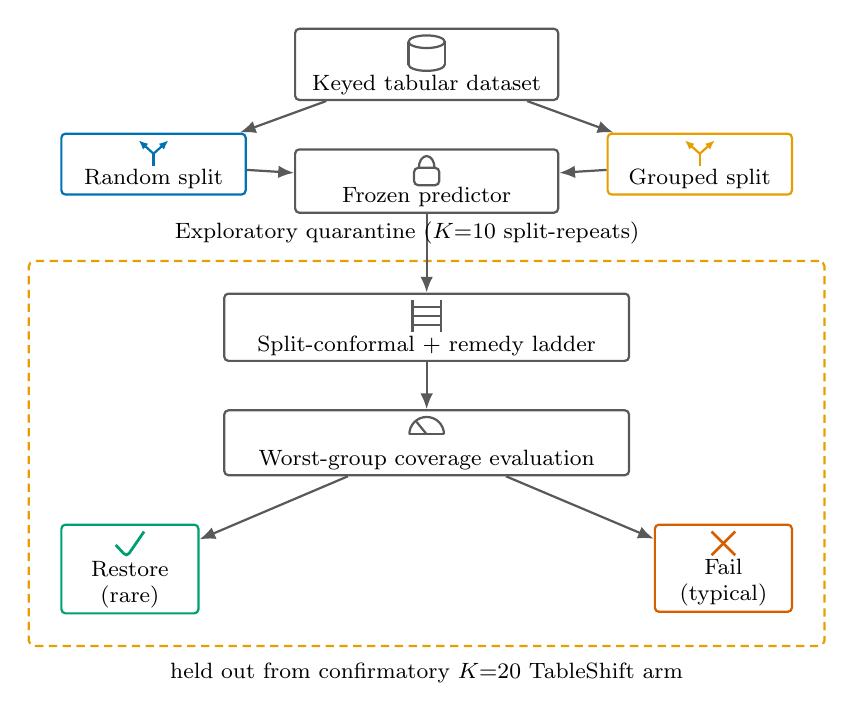
\begin{tikzpicture}[
    font=\fontsize{8}{9.5}\selectfont,
    node distance=4mm and 6mm,
    box/.style={draw=oiGrey, thick, rounded corners=1.5pt, align=center,
                fill=white, minimum height=6mm, text width=32mm, inner sep=2pt},
    splitbox/.style={box, text width=22mm},
    verdictbox/.style={box, text width=16mm, minimum height=6mm},
    arr/.style={-{Latex[length=2mm,width=1.6mm]}, thick, oiGrey},
    quarantine/.style={draw=oiOrange, thick, dash pattern=on 3pt off 2pt,
                        rounded corners=2pt, inner sep=2.5mm}
]

% -- Row 1: data
\node[box] (data) {\iconDB\\ Keyed tabular dataset};

% -- Row 2: split branch
\node[splitbox, below left=of data, draw=oiBlue] (rsplit)
  {\iconSplit{oiBlue}\\ Random split};
\node[splitbox, below right=of data, draw=oiOrange] (gsplit)
  {\iconSplit{oiOrange}\\ Grouped split};

% -- Row 3: frozen predictor
\node[box, below=6mm of data] (pred)
  {\iconLock\\ Frozen predictor};

% -- Row 4: conformal + remedy ladder
\node[box, below=10mm of pred, text width=50mm] (ladder)
  {\iconLadder\\ Split-conformal + remedy ladder};

% -- Row 5: worst-group coverage evaluation
\node[box, below=6mm of ladder, text width=50mm] (eval)
  {\iconGauge\\ Worst-group coverage evaluation};

% -- Row 6: verdicts
\node[verdictbox, below left=6mm and 3mm of eval, draw=oiGreen] (restore)
  {\iconCheck\\ Restore (rare)};
\node[verdictbox, below right=6mm and 3mm of eval, draw=oiVermillion] (fail)
  {\iconCross\\ Fail (typical)};

% -- arrows
\draw[arr] (data) -- (rsplit);
\draw[arr] (data) -- (gsplit);
\draw[arr] (rsplit) -- (pred);
\draw[arr] (gsplit) -- (pred);
\draw[arr] (pred) -- (ladder);
\draw[arr] (ladder) -- (eval);
\draw[arr] (eval) -- (restore);
\draw[arr] (eval) -- (fail);

% -- exploratory/confirmatory quarantine (black annotation text; the dashed
% border itself carries the orange color-coding, per the black-text-only rule)
\begin{scope}[on background layer]
  \node[quarantine, fit=(ladder)(eval)(restore)(fail), inner sep=4mm] (quar) {};
\end{scope}
\node[black, align=center, above=0.8mm of quar.north, xshift=-2.5mm, font=\fontsize{8}{9.5}\selectfont] (quarlabel)
  {Exploratory quarantine ($K{=}10$ split-repeats)};
\node[black, align=center, below=0.8mm of quar.south, font=\fontsize{8}{9.5}\selectfont] (quarnote)
  {held out from confirmatory $K{=}20$ TableShift arm};

\end{tikzpicture}
\end{document}
